\clearpage
\subsection{MSVC: x86 + \olly}
\myindex{\olly}

Тут даже проще:

\begin{figure}[H]
\centering
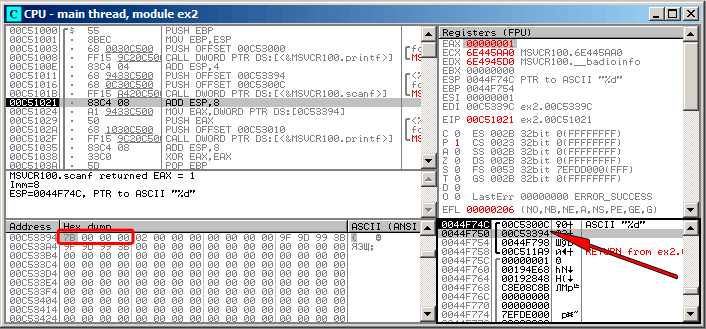
\includegraphics[scale=\FigScale]{patterns/04_scanf/2_global/ex2_olly_1.png}
\caption{\olly: после исполнения \scanf}
\label{fig:scanf_ex2_olly_1}
\end{figure}

Переменная хранится в сегменте данных.
Кстати, после исполнения инструкции \PUSH (заталкивающей адрес $x$) адрес появится в стеке, 
и на этом элементе можно нажать правой кнопкой, выбрать \q{Follow in dump}.
И в окне памяти слева появится эта переменная.

После того как в консоли введем 123, здесь появится \TT{0x7B}.

Почему самый первый байт это \TT{7B}?
По логике вещей, здесь должно было бы быть \TT{00 00 00 7B}.
Это называется \gls{endianness}, и в x86 принят формат \IT{little-endian}.
Это означает, что в начале записывается самый младший байт, а заканчивается самым старшим байтом.
Больше об этом: \myref{sec:endianness}.

Позже из этого места в памяти 32-битное значение загружается в \EAX и передается в \printf.

Адрес переменной $x$ в памяти \TT{0x00C53394}.

\clearpage
В \olly{} мы можем посмотреть карту памяти процесса (Alt-M) и увидим, что этот адрес
внутри PE-сегмента \TT{.data} нашей программы:

\begin{figure}[H]
\centering
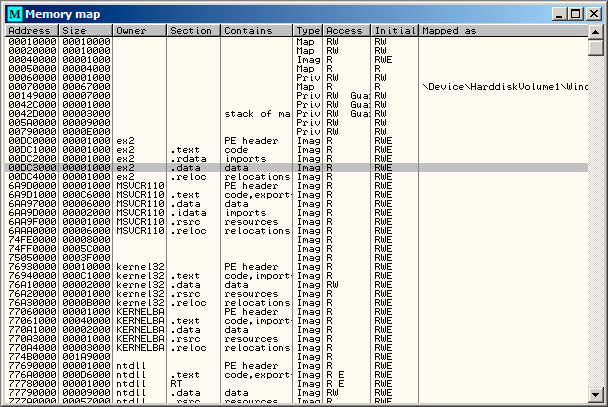
\includegraphics[scale=\FigScale]{patterns/04_scanf/2_global/ex2_olly_2.png}
\caption{\olly: карта памяти процесса}
\label{fig:scanf_ex2_olly_2}
\end{figure}
